\documentclass{standalone}
\usepackage{tikz}
\usetikzlibrary{patterns, positioning}


\begin{document}
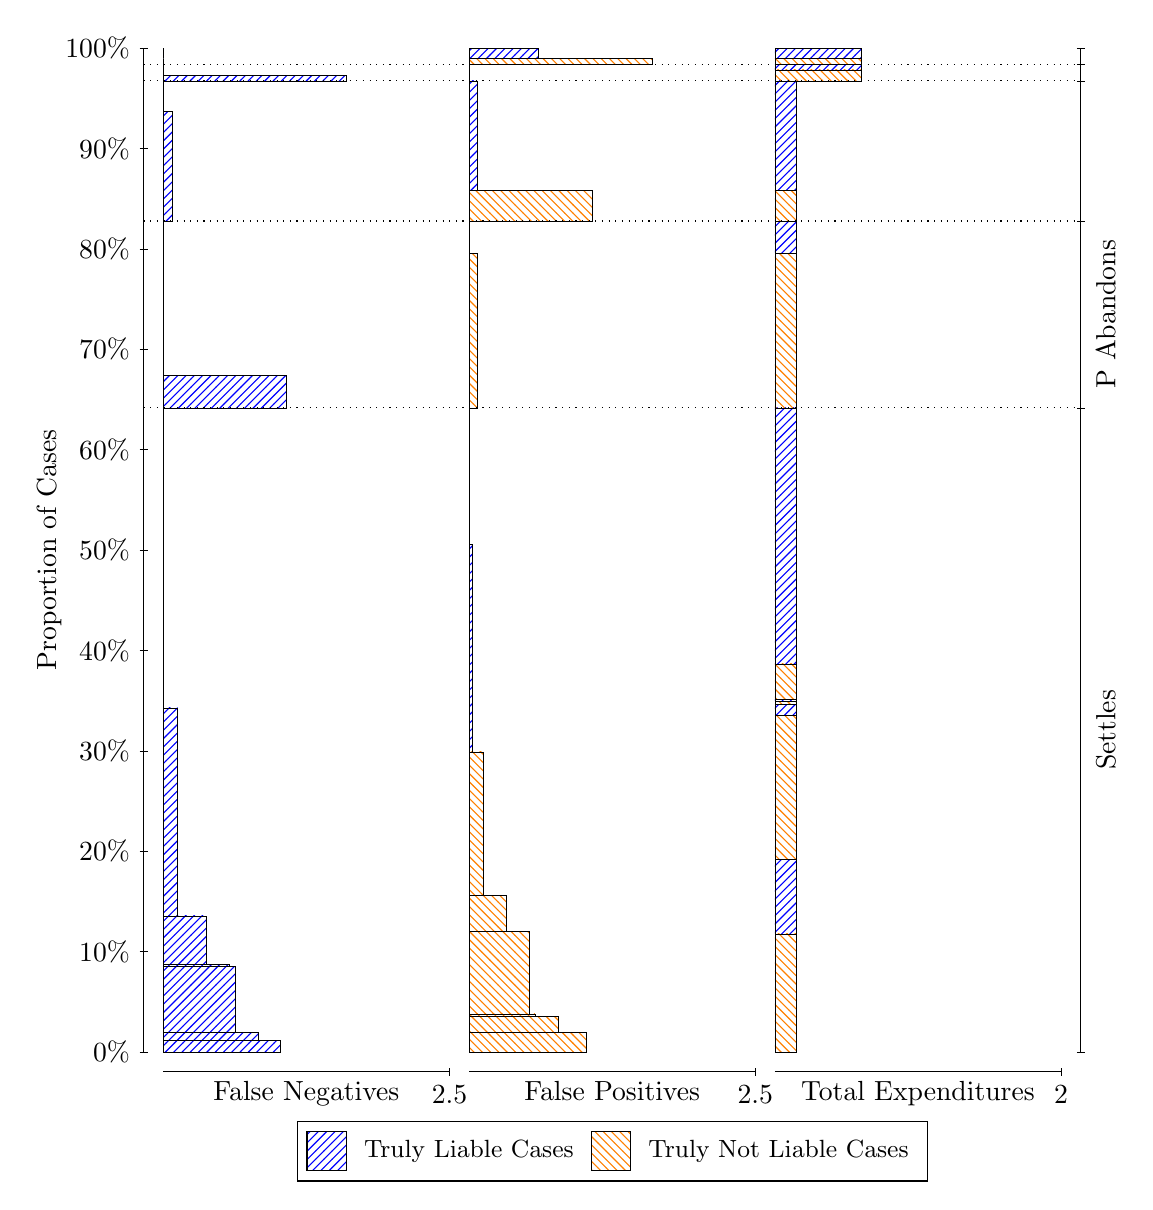
\begin{tikzpicture}
\draw[black, very thin] (1.5,1.75) -- (1.5,14.5);
\node[rotate=90, text=black, anchor=center] at (0.3, 8.125) {Proportion of Cases};
\draw[black, very thin] (1.45,1.75) -- (1.55,1.75);
\node[text=black, anchor=east] at (1.45, 1.75) {0\%};
\draw[black, very thin] (1.45,3.025) -- (1.55,3.025);
\node[text=black, anchor=east] at (1.45, 3.025) {10\%};
\draw[black, very thin] (1.45,4.3) -- (1.55,4.3);
\node[text=black, anchor=east] at (1.45, 4.3) {20\%};
\draw[black, very thin] (1.45,5.575) -- (1.55,5.575);
\node[text=black, anchor=east] at (1.45, 5.575) {30\%};
\draw[black, very thin] (1.45,6.85) -- (1.55,6.85);
\node[text=black, anchor=east] at (1.45, 6.85) {40\%};
\draw[black, very thin] (1.45,8.125) -- (1.55,8.125);
\node[text=black, anchor=east] at (1.45, 8.125) {50\%};
\draw[black, very thin] (1.45,9.4) -- (1.55,9.4);
\node[text=black, anchor=east] at (1.45, 9.4) {60\%};
\draw[black, very thin] (1.45,10.675) -- (1.55,10.675);
\node[text=black, anchor=east] at (1.45, 10.675) {70\%};
\draw[black, very thin] (1.45,11.95) -- (1.55,11.95);
\node[text=black, anchor=east] at (1.45, 11.95) {80\%};
\draw[black, very thin] (1.45,13.225) -- (1.55,13.225);
\node[text=black, anchor=east] at (1.45, 13.225) {90\%};
\draw[black, very thin] (1.45,14.5) -- (1.55,14.5);
\node[text=black, anchor=east] at (1.45, 14.5) {100\%};

\draw[black, very thin] (13.4,1.75) -- (13.4,14.5);
\draw[black, very thin] (13.35,1.75) -- (13.45,1.75);
\node[anchor=west] at (13.35, 1.75) {};
\draw[black, very thin] (13.35,9.9306) -- (13.45,9.9306);
\node[anchor=west] at (13.35, 9.9306) {};
\draw[black, very thin] (13.35,12.303) -- (13.45,12.303);
\node[anchor=west] at (13.35, 12.303) {};
\draw[black, very thin] (13.35,14.082) -- (13.45,14.082);
\node[anchor=west] at (13.35, 14.082) {};
\draw[black, very thin] (13.35,14.296) -- (13.45,14.296);
\node[anchor=west] at (13.35, 14.296) {};
\draw[black, very thin] (13.35,14.5) -- (13.45,14.5);
\node[anchor=west] at (13.35, 14.5) {};

\draw[black, very thin, pattern color=blue, pattern=north east lines] (1.75,1.75) rectangle (3.2397,1.8973);
\draw[black, very thin, pattern color=blue, pattern=north east lines] (1.75,1.8973) rectangle (2.949,2.0001);
\draw[black, very thin, pattern color=blue, pattern=north east lines] (1.75,2.0001) rectangle (2.6583,2.8419);
\draw[black, very thin, pattern color=blue, pattern=north east lines] (1.75,2.8419) rectangle (2.5857,2.8664);
\draw[black, very thin, pattern color=blue, pattern=north east lines] (1.75,2.8664) rectangle (2.295,3.477);
\draw[black, very thin, pattern color=blue, pattern=north east lines] (1.75,3.477) rectangle (1.9317,6.1191);
\draw[black, very thin, pattern color=orange, pattern=north west lines] (1.75,6.1191) rectangle (1.75,9.9306);
\draw[black, very thin, pattern color=blue, pattern=north east lines] (1.75,9.9306) rectangle (3.3123,10.344);
\draw[black, very thin, pattern color=orange, pattern=north west lines] (1.75,10.344) rectangle (1.75,12.303);
\draw[black, very thin, pattern color=blue, pattern=north east lines] (1.75,12.303) rectangle (1.859,13.692);
\draw[black, very thin, pattern color=orange, pattern=north west lines] (1.75,13.692) rectangle (1.75,14.082);
\draw[black, very thin, pattern color=blue, pattern=north east lines] (1.75,14.082) rectangle (4.0753,14.155);
\draw[black, very thin, pattern color=orange, pattern=north west lines] (1.75,14.155) rectangle (1.75,14.296);
\draw[black, very thin, pattern color=orange, pattern=north west lines] (1.75,14.296) rectangle (1.75,14.369);
\draw[black, very thin, pattern color=blue, pattern=north east lines] (1.75,14.369) rectangle (1.75,14.5);
\draw[black, very thin, pattern color=orange, pattern=north west lines] (5.6333,1.75) rectangle (7.123,2.0016);
\draw[black, very thin, pattern color=orange, pattern=north west lines] (5.6333,2.0016) rectangle (6.7597,2.2036);
\draw[black, very thin, pattern color=orange, pattern=north west lines] (5.6333,2.2036) rectangle (6.469,2.2345);
\draw[black, very thin, pattern color=orange, pattern=north west lines] (5.6333,2.2345) rectangle (6.3963,3.2786);
\draw[black, very thin, pattern color=orange, pattern=north west lines] (5.6333,3.2786) rectangle (6.1057,3.7352);
\draw[black, very thin, pattern color=orange, pattern=north west lines] (5.6333,3.7352) rectangle (5.815,5.5615);
\draw[black, very thin, pattern color=blue, pattern=north east lines] (5.6333,5.5615) rectangle (5.6697,8.2036);
\draw[black, very thin, pattern color=blue, pattern=north east lines] (5.6333,8.2036) rectangle (5.6333,9.9306);
\draw[black, very thin, pattern color=orange, pattern=north west lines] (5.6333,9.9306) rectangle (5.7423,11.89);
\draw[black, very thin, pattern color=blue, pattern=north east lines] (5.6333,11.89) rectangle (5.6333,12.303);
\draw[black, very thin, pattern color=orange, pattern=north west lines] (5.6333,12.303) rectangle (7.1957,12.693);
\draw[black, very thin, pattern color=blue, pattern=north east lines] (5.6333,12.693) rectangle (5.7423,14.082);
\draw[black, very thin, pattern color=orange, pattern=north west lines] (5.6333,14.082) rectangle (5.6333,14.223);
\draw[black, very thin, pattern color=blue, pattern=north east lines] (5.6333,14.223) rectangle (5.6333,14.296);
\draw[black, very thin, pattern color=orange, pattern=north west lines] (5.6333,14.296) rectangle (7.9587,14.369);
\draw[black, very thin, pattern color=blue, pattern=north east lines] (5.6333,14.369) rectangle (6.5053,14.5);
\draw[black, very thin, pattern color=orange, pattern=north west lines] (9.5167,1.75) rectangle (9.7892,3.2508);
\draw[black, very thin, pattern color=blue, pattern=north east lines] (9.5167,3.2508) rectangle (9.7892,4.1954);
\draw[black, very thin, pattern color=orange, pattern=north west lines] (9.5167,4.1954) rectangle (9.7892,6.0216);
\draw[black, very thin, pattern color=blue, pattern=north east lines] (9.5167,6.0216) rectangle (9.7892,6.1689);
\draw[black, very thin, pattern color=orange, pattern=north west lines] (9.5167,6.1689) rectangle (9.7892,6.1998);
\draw[black, very thin, pattern color=blue, pattern=north east lines] (9.5167,6.1998) rectangle (9.7892,6.2243);
\draw[black, very thin, pattern color=orange, pattern=north west lines] (9.5167,6.2243) rectangle (9.7892,6.6778);
\draw[black, very thin, pattern color=blue, pattern=north east lines] (9.5167,6.6778) rectangle (9.7892,9.9306);
\draw[black, very thin, pattern color=orange, pattern=north west lines] (9.5167,9.9306) rectangle (9.7892,11.89);
\draw[black, very thin, pattern color=blue, pattern=north east lines] (9.5167,11.89) rectangle (9.7892,12.303);
\draw[black, very thin, pattern color=orange, pattern=north west lines] (9.5167,12.303) rectangle (9.7892,12.693);
\draw[black, very thin, pattern color=blue, pattern=north east lines] (9.5167,12.693) rectangle (9.7892,14.082);
\draw[black, very thin, pattern color=orange, pattern=north west lines] (9.5167,14.082) rectangle (10.607,14.223);
\draw[black, very thin, pattern color=blue, pattern=north east lines] (9.5167,14.223) rectangle (10.607,14.296);
\draw[black, very thin, pattern color=orange, pattern=north west lines] (9.5167,14.296) rectangle (10.607,14.369);
\draw[black, very thin, pattern color=blue, pattern=north east lines] (9.5167,14.369) rectangle (10.607,14.5);
\draw[black, dotted] (1.5,9.9306) -- (13.4,9.9306);
\draw[black, dotted] (1.5,12.303) -- (13.4,12.303);
\draw[black, dotted] (1.5,14.082) -- (13.4,14.082);
\draw[black, dotted] (1.5,14.296) -- (13.4,14.296);
\draw[black, very thin] (1.75,1.5) -- (5.3833,1.5);
\node[text=black, anchor=north] at (3.5667, 1.5) {False Negatives};
\draw[black, very thin] (5.3833,1.45) -- (5.3833,1.55);
\node[text=black, anchor=north] at (5.3833, 1.45) {2.5};

\draw[black, very thin] (5.6333,1.5) -- (9.2667,1.5);
\node[text=black, anchor=north] at (7.45, 1.5) {False Positives};
\draw[black, very thin] (9.2667,1.45) -- (9.2667,1.55);
\node[text=black, anchor=north] at (9.2667, 1.45) {2.5};

\draw[black, very thin] (9.5167,1.5) -- (13.15,1.5);
\node[text=black, anchor=north] at (11.333, 1.5) {Total Expenditures};
\draw[black, very thin] (13.15,1.45) -- (13.15,1.55);
\node[text=black, anchor=north] at (13.15, 1.45) {2};

\node[text=black, centered, rotate=90] at (13.72, 5.8403) {Settles};
\node[text=black, centered, rotate=90] at (13.72, 11.117) {P Abandons};




\draw (7.449999999999999,1.5) node[draw=none] (baseCoordinate) {};
\begin{scope}[align=center]
        \matrix[scale=0.5, draw=black, below=0.5cm of baseCoordinate, nodes={draw}, column sep=0.1cm]{
            \node[rectangle, draw, minimum width=0.5cm, minimum height=0.5cm, pattern color=blue, pattern=north east lines] {}; &
            \node[draw=none, font=\small, text=black] (B) {Truly Liable Cases}; &
            \node[rectangle, draw, minimum width=0.5cm, minimum height=0.5cm, pattern color=orange, pattern=north west lines] {}; &
            \node[draw=none, font=\small, text=black] (B) {Truly Not Liable Cases}; \\
            };
\end{scope}

\end{tikzpicture}
\end{document}